\documentclass[12pt]{beamer}

\usepackage[utf8]{inputenc}
\usepackage{graphics}
\usepackage{listings}

\usepackage{array,booktabs}

\usetheme{Madrid}
\usecolortheme{beaver}

% custom commands
\newcommand{\nologo}{\setbeamertemplate{logo}{}} % set logo to empty

\title{Kubernetes}
\author{Arun}
\date{\today}


\logo{
\includegraphics[height=1.0cm]{images/k8s.png}}

\begin{document}
    \frame{\titlepage}
    \begin{frame}
        \begin{center}
            \huge{First bit of basics}
        \end{center}
    \end{frame}

    \begin{frame}
        \begin{center}
            \frametitle{First bit of basics}
            \begin{itemize}
                \item pods
                \item deployment
                \item service
                \item horizontal pot autoscaler (HPA)
            \end{itemize}
        \end{center}
    \end{frame}

    \begin{frame}
        \begin{center}
            \huge{Before k8s}
        \end{center}
    \end{frame}

    \begin{frame}
        \frametitle{Before k8s}
        \begin{itemize}
            \item 600+ servers
            \item External load balancers see 5K+ requests per $second$
            \item Internal Amplification of 8x to 12x
        \end{itemize}
    \end{frame}

    \begin{frame}
        \frametitle{Kubernetes}
        \begin{columns}
            \column{0.4\textwidth}
            \begin{center}
                
\includegraphics[width=1\textwidth]{images/k8s.png}
            \end{center}

            \column{0.6\textwidth}
            \begin{itemize}
                \item Partial Kubernetes deployment since Oct, 2016
                \item Full Production deployment since Nov, 2016
                \item Using Google Container Engine
                \pause
                \item 5+ Clusters
                \item 75+ deployments
                \item 500+ containers $($At Peak$)$
                \pause
                \item All new services directly onboard to kubernetes
                \item Autoscaled on CPU targets
            \end{itemize}
        \end{columns}
    \end{frame}

    \begin{frame}
        \frametitle{Kubernetes}
        \begin{columns}
            \column{0.4\textwidth}
            \begin{center}
                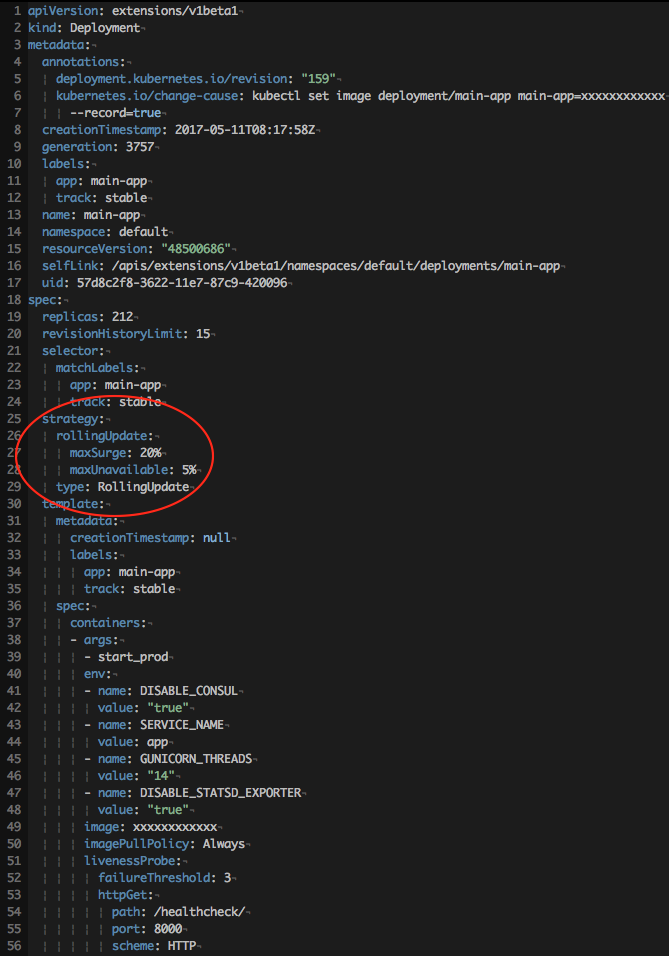
\includegraphics[width=1\textwidth]{images/kubernetes-config-rolling.png}<1>
                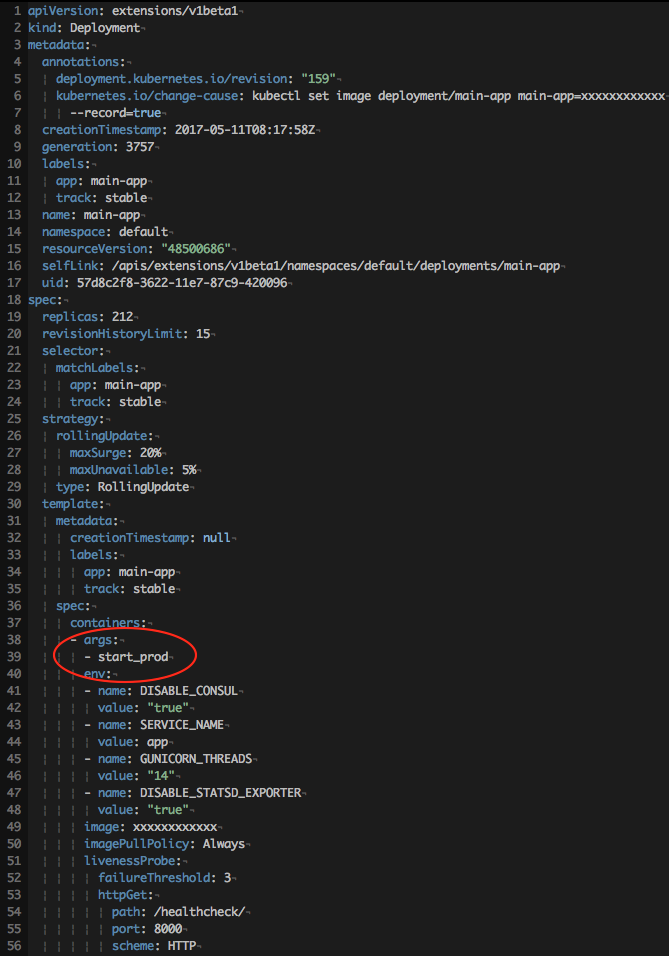
\includegraphics[width=1\textwidth]{images/kubernetes-config-command.png}<2>
                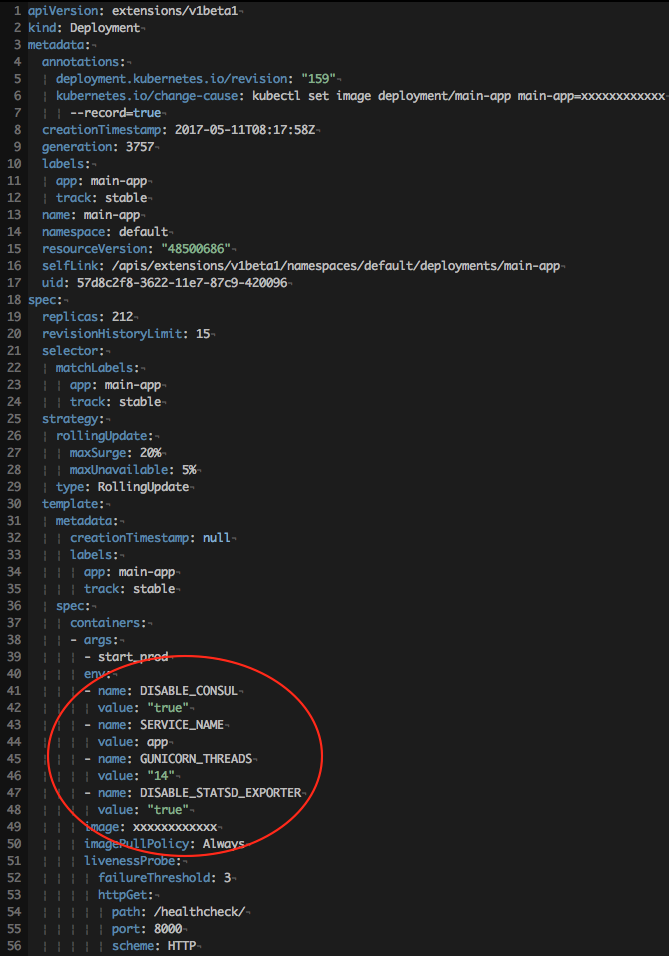
\includegraphics[width=1\textwidth]{images/kubernetes-config-env.png}<3>
                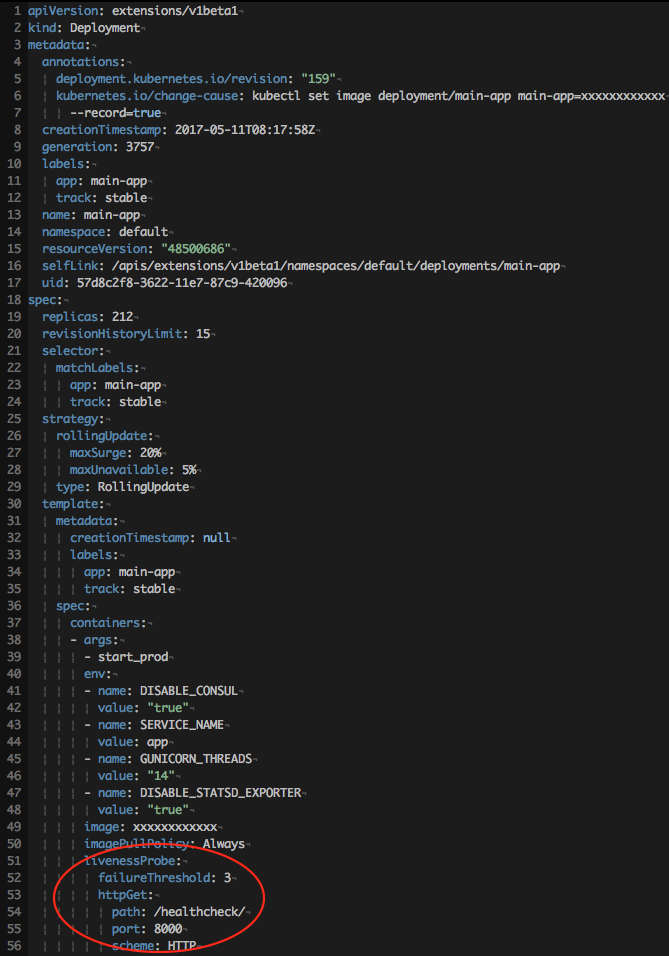
\includegraphics[width=1\textwidth]{images/kubernetes-config-health.png}<4>
            \end{center}

            \column{0.6\textwidth}
            \begin{itemize}
                \item Rolling updates across containers
                \pause
                \item Custom commands to run same container across dev/stage/prod environments
                \pause
                \item Environment variables to override 'config-service' values
                \pause
                \item Liveness and Readiness checks are must!
            \end{itemize}
        \end{columns}
    \end{frame}

    \begin{frame}
        \frametitle{Kubernetes Autoscaling}
        \begin{center}
            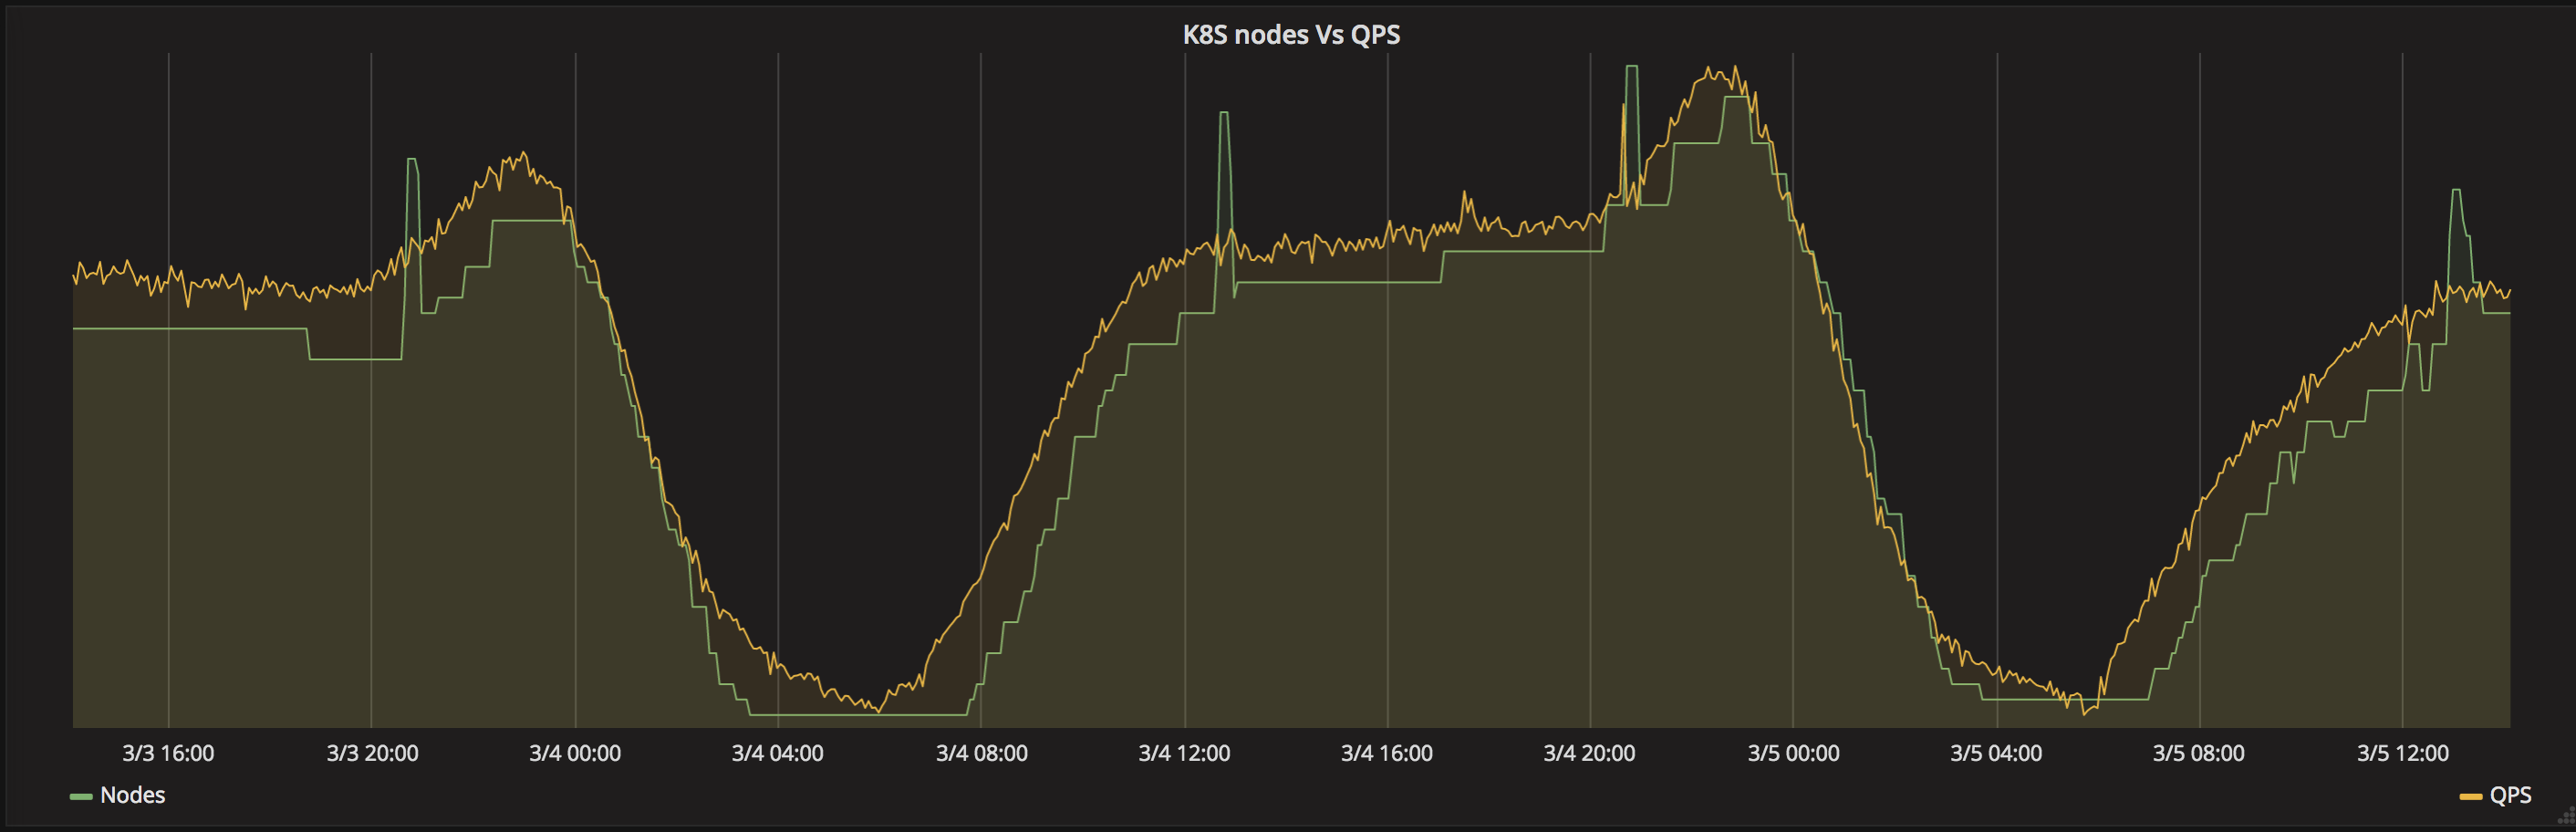
\includegraphics[width=1\textwidth]{images/kubernetes-auto.png}
        \end{center}
    \end{frame}

    \begin{frame}
        \frametitle{Kubernetes}
        \begin{columns}
            \column{0.4\textwidth}
            \begin{center}
                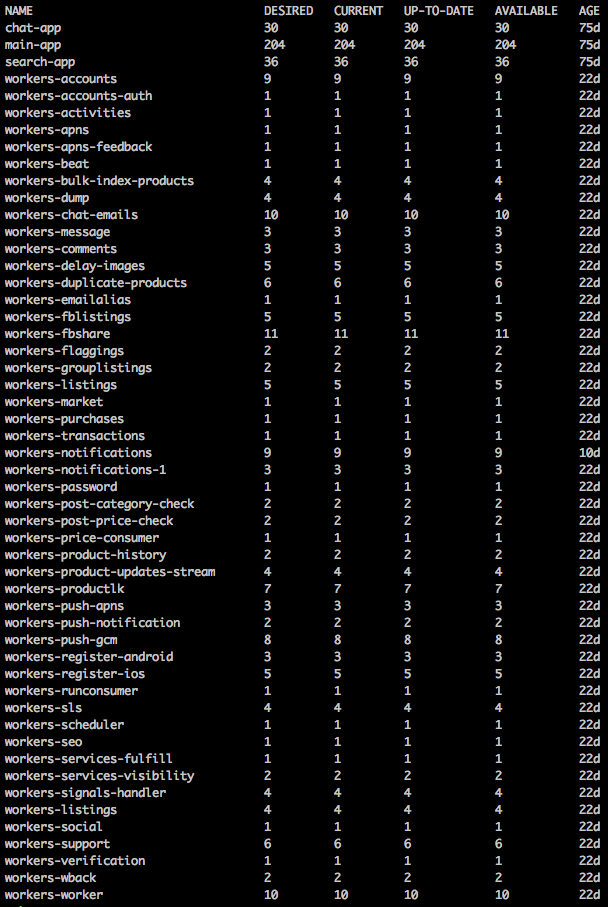
\includegraphics[width=1\textwidth]{images/kubernetes-deploy.png}
            \end{center}

            \column{0.6\textwidth}
            \begin{itemize}
                \item Not using \textbf{K8S Ingress/Service}
                    \pause
                \item Config-Service as DaemonSet
                \item Containers get registered on Config-Service $(NodePort)$ from health check
                    \pause
                \item No change in existing architecture needed
                \item Service discovery from Internal/External load balancers
            \end{itemize}
        \end{columns}
    \end{frame}

    \begin{frame}
        \frametitle{Kubernetes}
        \begin{center}
            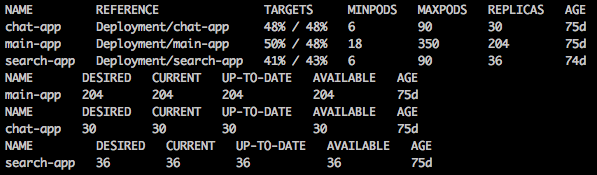
\includegraphics[width=0.7\textwidth]{images/kubernetes-status.png}
        \end{center}
        \begin{itemize}
            \item 'Config-Service' allows us to have hybrid model
            \item Services can be deployed in multiple clusters
            \item Instance groups can coexist with Kubernetes
            \pause
            \item Instances run the same container image
            \pause
            \item Recovery mechanism / Transitioning
            %\pause
            %\item Instance group size set to zero $($Fully on K8S$)$
            \pause
            \item Easy Migration - Create new K8S cluster and terminate old cluster
        \end{itemize}
    \end{frame}

    \begin{frame}
        \frametitle{Kubernetes}
        %\begin{columns}
            %\column{0.4\textwidth}
            \begin{center}
                
\includegraphics[height=0.4\textheight]{images/envoy-logo.png}<1>
                
\includegraphics[height=0.4\textheight]{images/prometheus.jpg}<2>
                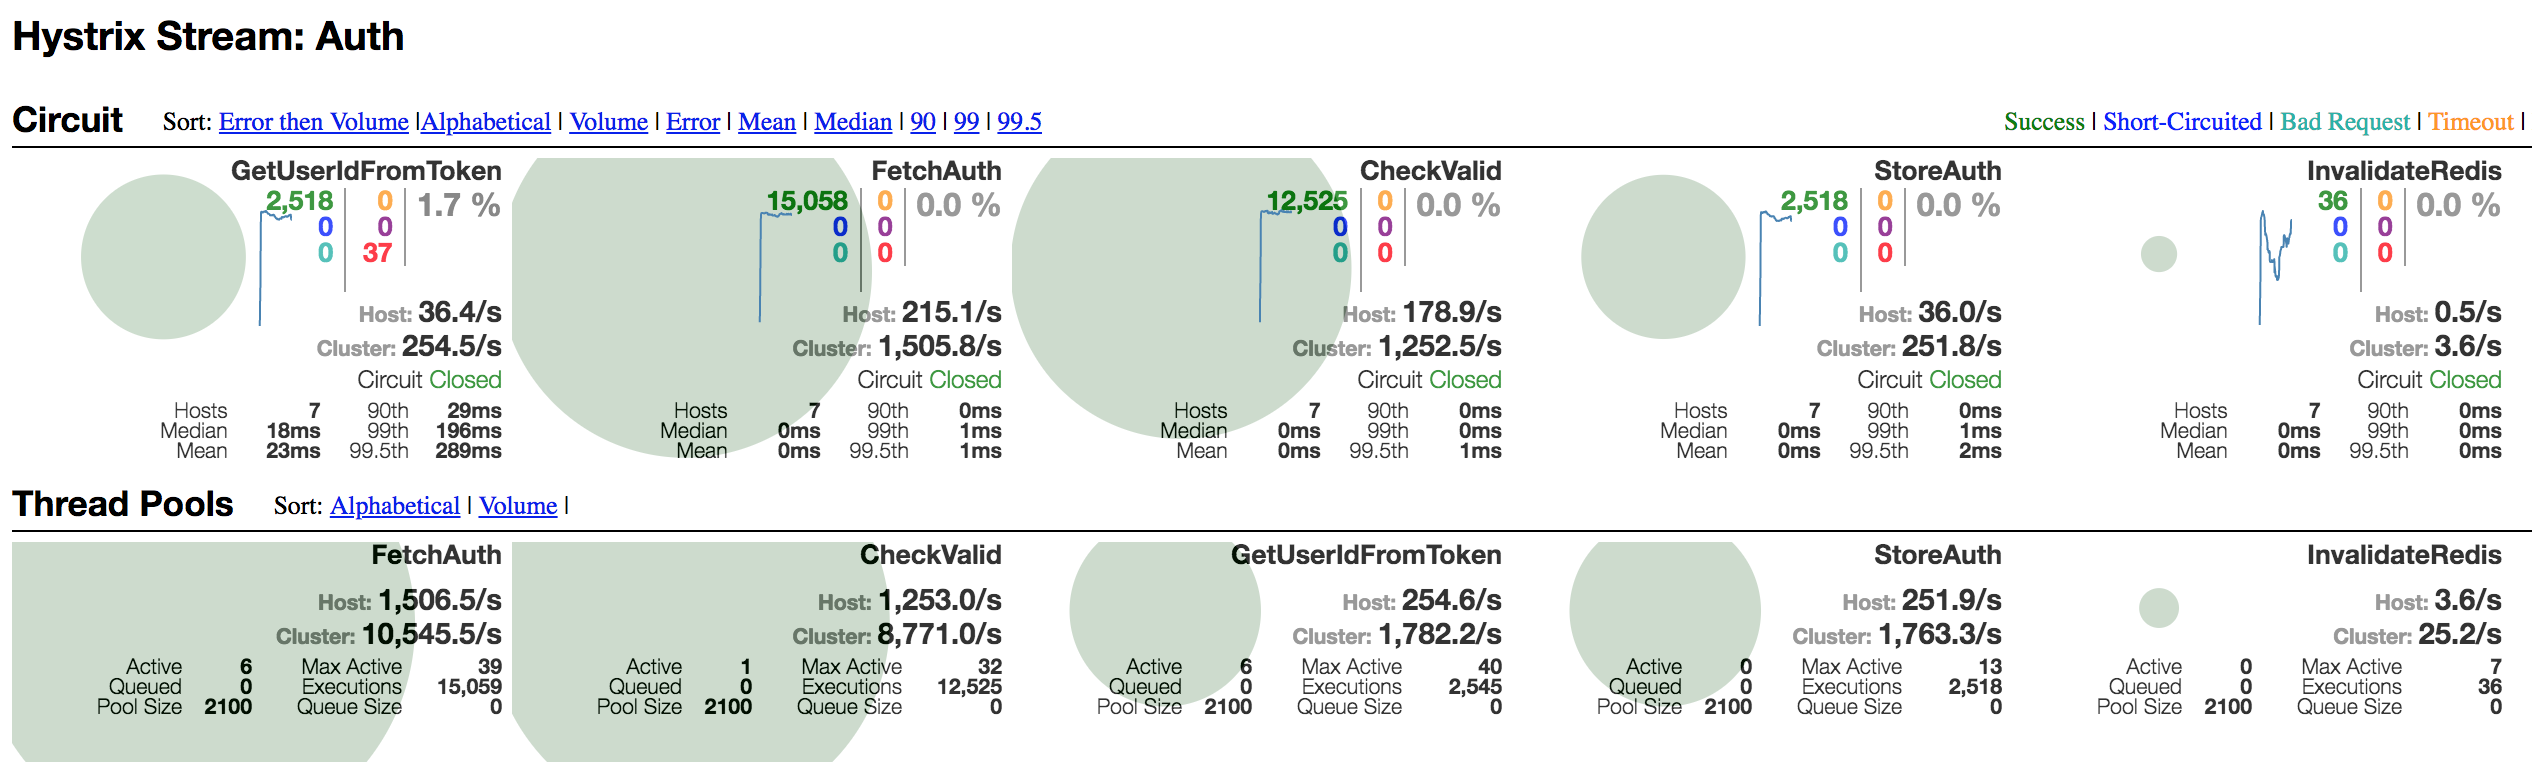
\includegraphics[height=0.4\textheight]{images/hystrix.png}<3>
                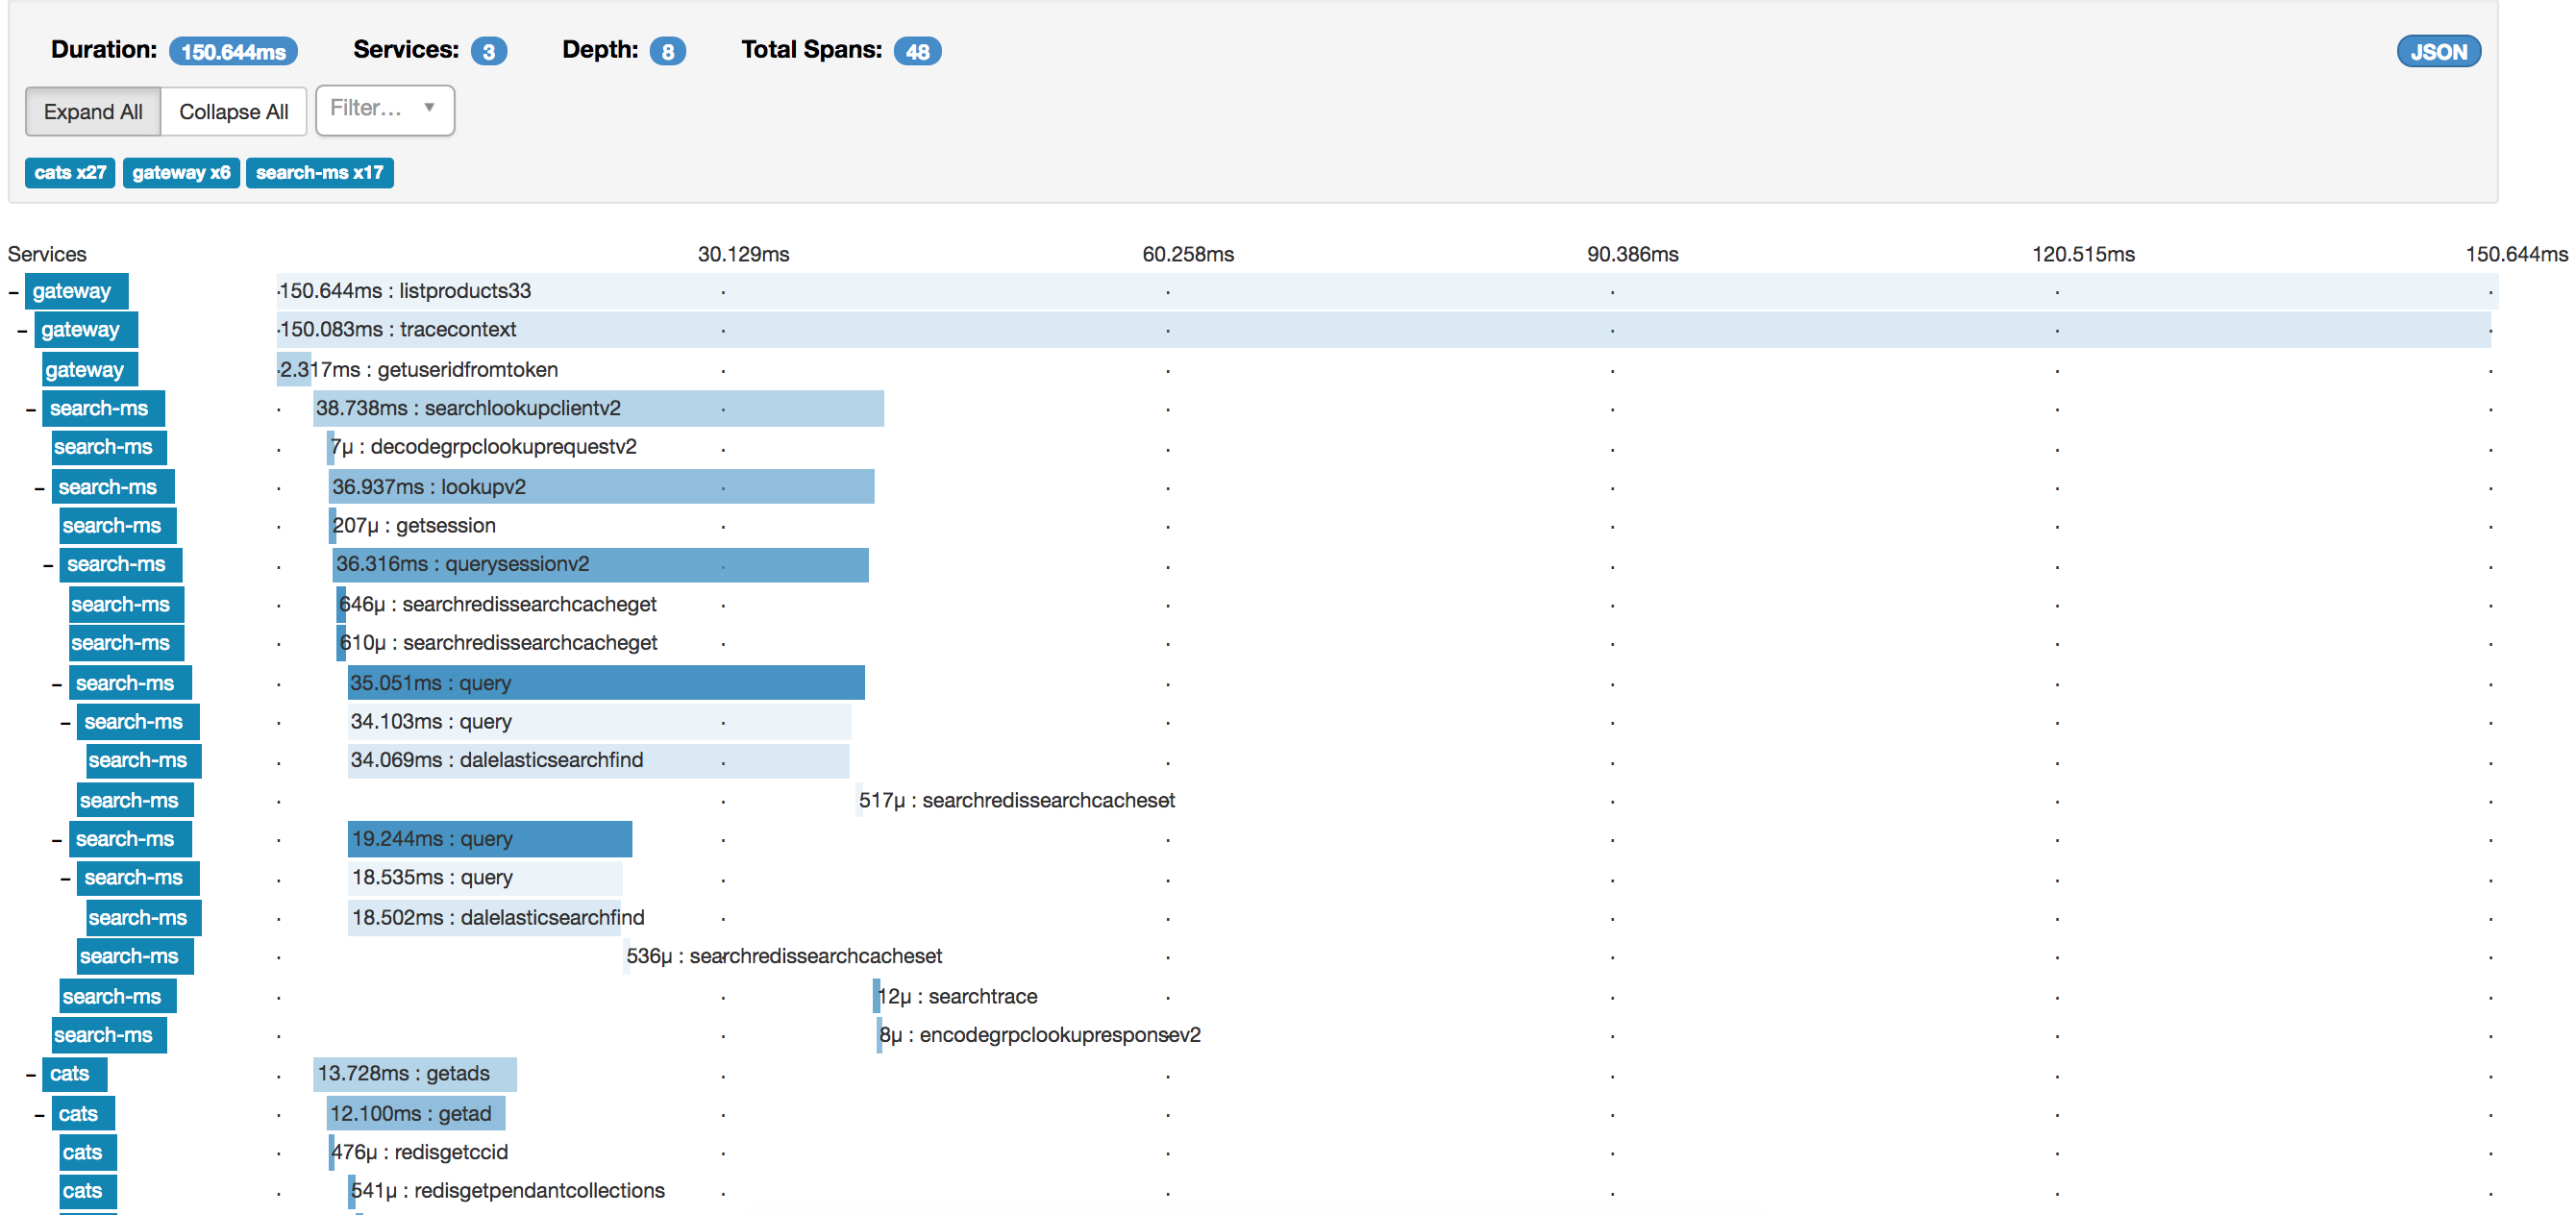
\includegraphics[height=0.5\textheight]{images/zipkin.png}<4>
            \end{center}

            %\column{0.6\textwidth}
            \begin{itemize}
                \item Envoy for communication between micro-services $($gRPC$)$
                \pause
                \item Prometheus for monitoring
                \pause
                \item Turbine for hystrix stream aggregation
                \pause
                \item Zipkin Spans are written to external kafka
            \end{itemize}
        %\end{columns}
    \end{frame}

    \begin{frame}
        \frametitle{Deployment Pipeline}
        \begin{center}
            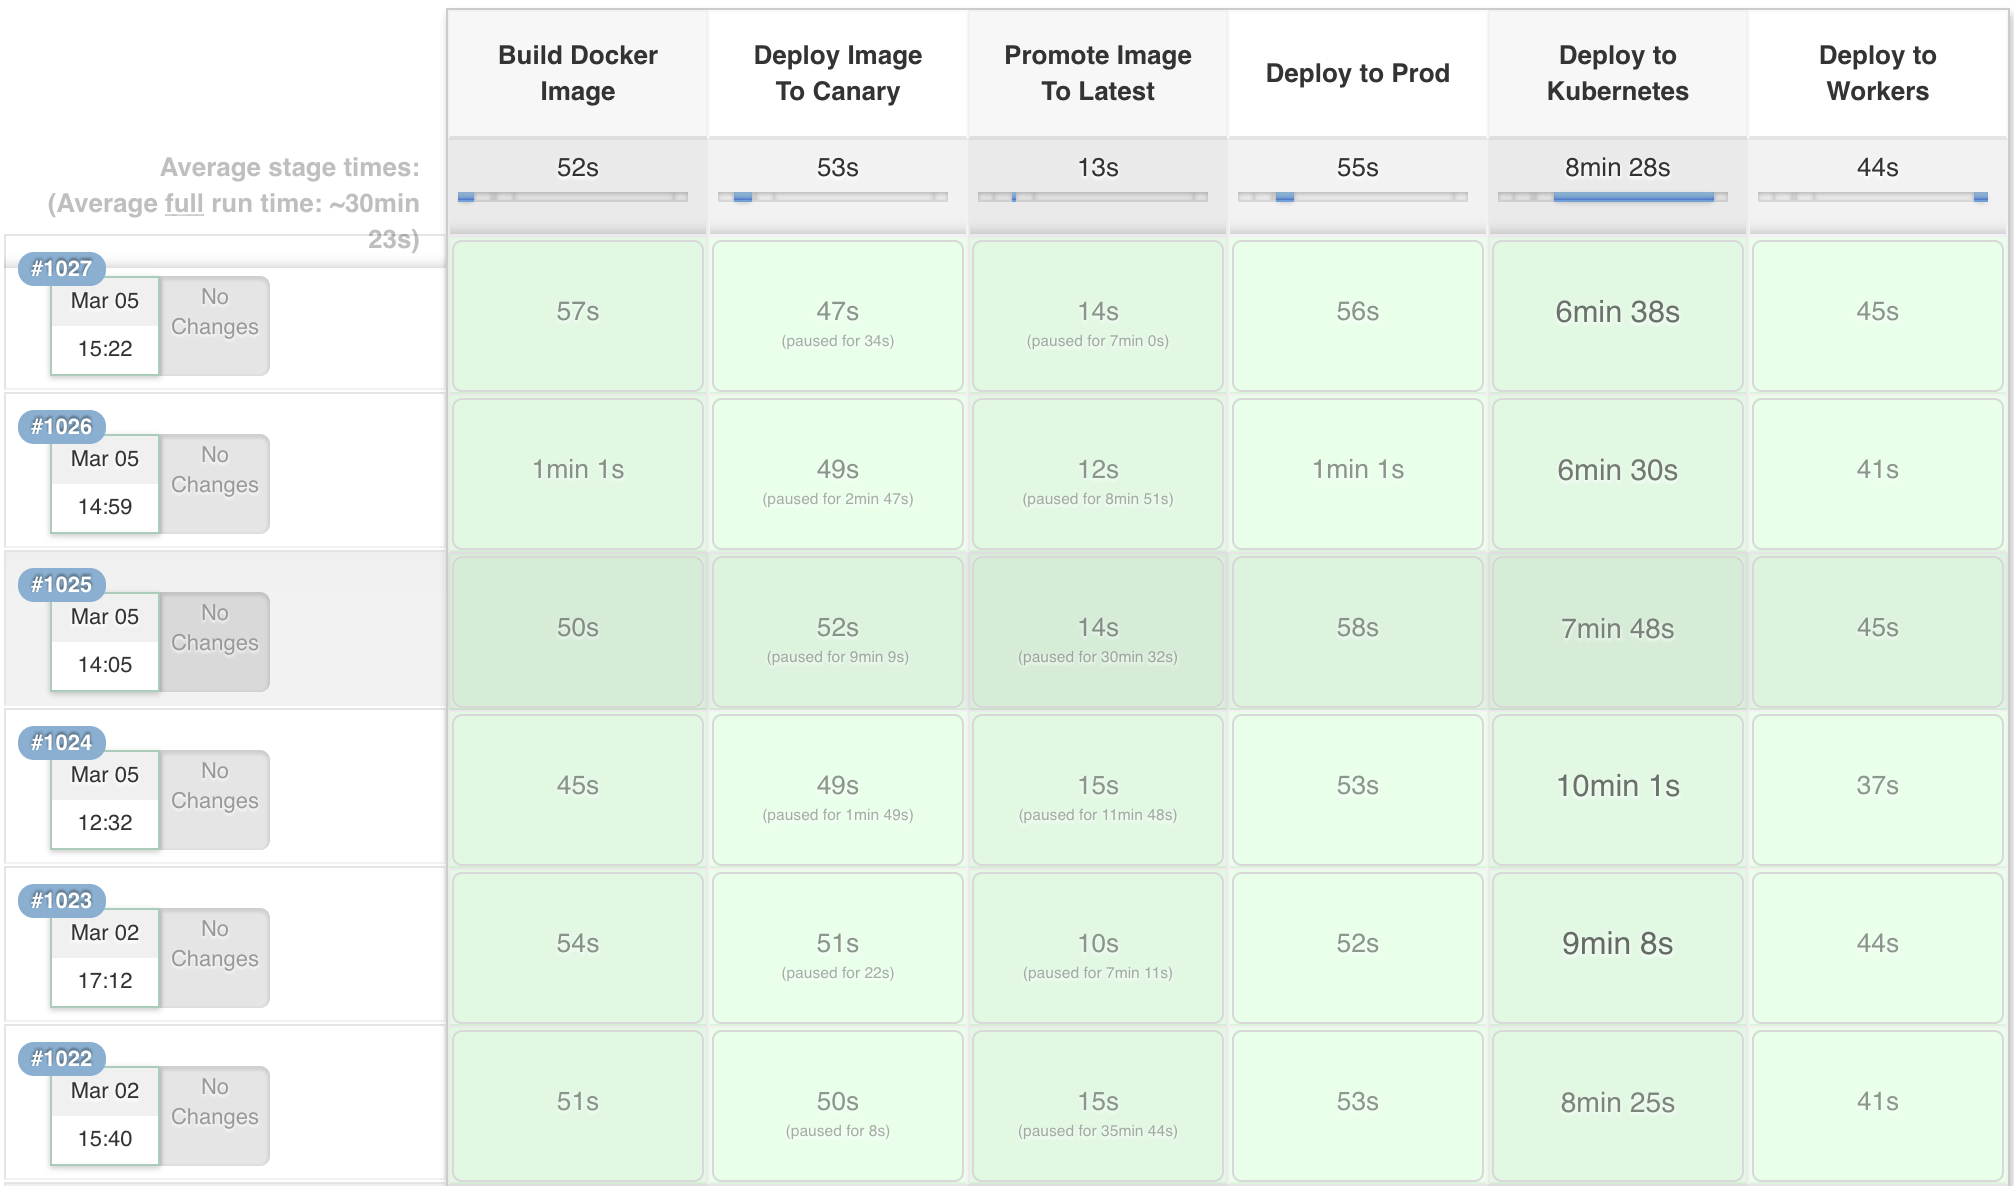
\includegraphics[width=1.00\textwidth]{images/pipeline.png}
        \end{center}
    \end{frame}

    \begin{frame}
        \frametitle{Thank You}
        \begin{table}[h!]
        \centering
                \begin{tabular}{ c }
                    \\
                    \\
                    \\
                    \\
                        \huge{Q\&A}\\
                        \\
                        \\
                        \\
                        \\
                        \\
                        \\
                \end{tabular}
        \end{table}
    \end{frame}
\end{document}
